\documentclass[tikz, border=4pt]{standalone}
\usepackage{amsmath}
\usetikzlibrary{arrows.meta,calc}

\begin{document}
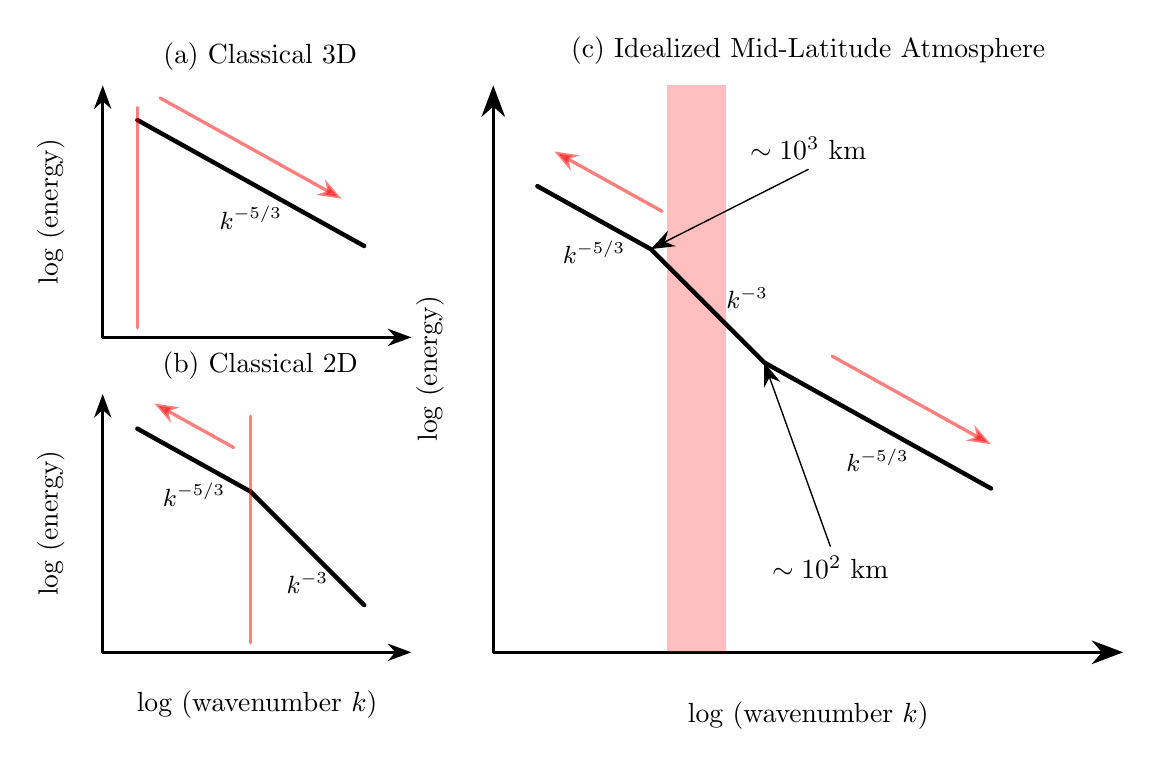
\begin{tikzpicture}[
  scale=.8,
    line cap=round,
    line join=round,
    spectrum/.style={line width=1.6pt},
    annot/.style={-{Stealth[length=3mm, width=2.2mm]}, line width=0.5pt},
    cascadearrow/.style={red, opacity=.5, line width=1.2pt,
    -{Stealth[length=3mm, width=2.2mm]}},
    scalearrow/.style={-{Stealth[length=3mm, width=2.2mm]}, line width=0.5pt}
  ]

% common slope geometry so all panels use the same actual angles
\def\dx{1.8}
\def\dyfive{1.0}
\def\dythree{1.8}

% ============================================================
% LEFT TOP PANEL: classical 3D spectrum ~ k^{-5/3}
% ============================================================
\begin{scope}[shift={(0,4.9)}]
  \node at (2.5,4.55) {(a) Classical 3D};

  \draw[-{Stealth[length=3mm, width=2.2mm]}, line width=0.9pt]
    (0,0.1) -- (0,4.1)
    node[midway, left=10pt, rotate=90, anchor=south] {log (energy)};
  \draw[-{Stealth[length=3mm, width=2.2mm]}, line width=0.9pt]
    (0,0.1) -- (4.9,0.1)
    node[midway, below=10pt] {};

  \coordinate (A3) at (0.55,3.55);
  \coordinate (B3) at ($(A3)+(\dx,-\dyfive)$);
  \coordinate (C3) at ($(B3)+(\dx,-\dyfive)$);

  \draw[spectrum] (A3) -- (B3) -- (C3);

  % red injection marker
  \draw[red, opacity=.5, line width=1.2pt]
    (0.55,0.25) -- (0.55,3.75);

% arrow parallel to spectrum
\draw[cascadearrow]
  ($(A3)!0.20!(B3)+(0,0.55)$)
  --
  ($(B3)!0.80!(C3)+(0,0.55)$);

% \node[red!70!black,font=\scriptsize]
%   at ($(A3)!0.5!(C3)+(0,0.95)$)
%   {energy cascade};

  % slope label BELOW spectrum
  \node[font=\small]
    at ($(A3)!0.5!(C3)+(0,-0.55)$)
    {$k^{-5/3}$};
\end{scope}

% ============================================================
% LEFT BOTTOM PANEL: classical 2D spectrum with kink
% ============================================================
\begin{scope}[shift={(0,0)}]
  \node at (2.5,4.55) {(b) Classical 2D};

  \draw[-{Stealth[length=3mm, width=2.2mm]}, line width=0.9pt]
    (0,0) -- (0,4.1)
    node[midway, left=10pt, rotate=90, anchor=south] {log (energy)};
  \draw[-{Stealth[length=3mm, width=2.2mm]}, line width=0.9pt]
    (0,0) -- (4.9,0)
    node[midway, below=10pt] {log (wavenumber $k$)};

  \coordinate (A2) at (0.55,3.55);
  \coordinate (K2) at ($(A2)+(\dx,-\dyfive)$);
  \coordinate (B2) at ($(K2)+(\dx,-\dythree)$);

  \draw[spectrum] (A2) -- (K2) -- (B2);

  % red injection marker at kink
  \draw[red, opacity=.5, line width=1.2pt] (2.35,0.15) -- (2.35,3.75);

% inverse energy cascade
\draw[cascadearrow]
  ($(K2)!0.15!(A2)+(0,0.55)$)
  --
  ($(A2)!0.15!(K2)+(0,0.55)$);

% \node[red!70!black,font=\scriptsize]
%   at ($(A2)!0.5!(K2)+(0,0.95)$)
%   {energy};

  % % forward enstrophy cascade
  % \draw[cascadearrow]
  %   (2.45,3.95) -- (4.15,3.95);

  % \node[red!70!black,font=\scriptsize]
  %   at (3.45,4.25)
  %   {enstrophy};

  % slope labels below spectrum
  \node[font=\small]
    at ($(A2)!0.5!(K2)+(0,-0.55)$)
    {$k^{-5/3}$};

  \node[font=\small]
    at ($(K2)!0.5!(B2)+(0,-0.55)$)
    {$k^{-3}$};
\end{scope}

% ============================================================
% RIGHT PANEL: atmospheric kinetic energy spectrum
% ============================================================
\begin{scope}[shift={(6.2,0)}]
  \node at (5.0,9.55) {(c) Idealized Mid-Latitude Atmosphere};

  % Axes
  \draw[-{Stealth[length=4mm, width=3mm]}, line width=1pt]
    (0,0) -- (0,9)
    node[midway, left=14pt, rotate=90, anchor=south] {log (energy)};
  \draw[-{Stealth[length=4mm, width=3mm]}, line width=1pt]
    (0,0) -- (10,0)
    node[midway, below=14pt] {log (wavenumber $k$)};

  % Broad fading injection band around first kink (synoptic forcing range)
  % \fill[red, opacity=.03] (1.2,0) rectangle (4.3,9);
  % \fill[red, opacity=.05] (1.45,0) rectangle (4.05,9);
  % \fill[red, opacity=.08] (1.75,0) rectangle (3.75,9);
  % \fill[red, opacity=.12] (2.05,0) rectangle (3.45,9);
  \fill[red, opacity=.25] (2.75,0) rectangle (3.7,9);

  % Spectrum with common slopes
  \coordinate (S0) at (0.7,7.4);
  \coordinate (S1) at ($(S0)+(\dx,-\dyfive)$);
  \coordinate (S2) at ($(S1)+(\dx,-\dythree)$);
  \coordinate (S3) at ($(S2)+(\dx,-\dyfive)$);
  \coordinate (S4) at ($(S3)+(\dx,-\dyfive)$);

  \draw[spectrum] (S0) -- (S1) -- (S2) -- (S3) -- (S4);

\draw[cascadearrow]
  ($(S1)!-0.1!(S0)+(0,0.7)$)
  --
  ($(S0)!0.15!(S1)+(0,0.7)$);

  % \draw[cascadearrow]
  % ($(S1)!0.15!(S2)+(0,0.7)$)
  % --
  % ($(S2)!0.15!(S1)+(0,0.7)$);

\draw[cascadearrow]
  ($(S2)!0.3!(S4)+(0,0.7)$)
  --
  ($(S4)!0!(S2)+(0,0.7)$);

% \node[red!70!black,font=\scriptsize]
%   at ($(S0)!0.5!(S1)+(0,1.1)$)
%   {inverse cascade};

  % % downscale transfer from forcing range
  % \draw[cascadearrow]
  %   (3.0,8.15) -- (8.8,8.15);

  % \node[red!70!black,font=\scriptsize]
  %   at (1.8,8.45)
  %   {inverse cascade};

  % \node[red!70!black,font=\scriptsize]
  %   at (5.9,8.45)
  %   {forward cascade};

  % slope labels
    \node[font=\small]
    at ($(S0)!0.5!(S1)+(0,-0.55)$)
    {$k^{-5/3}$};
    \node[font=\small]
    at ($(S1)!0.85!(S2)+(0,+0.75)$)
    {$k^{-3}$};
        \node[font=\small]
    at ($(S2)!0.5!(S4)+(0,-0.55)$)
    {$k^{-5/3}$};

  % scale annotations at the kinks / ranges
  \node (l1) at (5,8) {$\sim 10^3$ km};
  \draw[scalearrow] (l1.south) -- (S1);

  \node (l2) at (5.35,1.35) {$\sim 10^2$ km};
  \draw[scalearrow] (l2.north) -- (S2);

  % \node (l3) at (7.75,1.05) {kms};
  % \draw[scalearrow] (l3.north) -- (S3);
\end{scope}

\end{tikzpicture}
\end{document}